\documentclass{article}
\usepackage{graphicx}
\title{Installation Instructions for modem\_reset board}
\author{Daniel Soto}
\date{\today}

\begin{document}
\maketitle

\section{Programming}
Programming of the ATmega8U2 chip was performed before board was shipped.


\section{Installation}

\subsection{Microcontroller Board}
The microcontroller board needs three connections made.
Connection 1 is between the USB hub and the mini-USB connector via the included
USB cable.
Connection two is between the ground pins of the microcontroller board and the
modem board.  This connection is made via the terminal block.
Connection three is between the PD0 pin of the microcontroller board and the 
ON pin of the modem board.
These connections are shown in Figure \ref{schematic}.
The microcontroller connection points are shown in Figure \ref{microcontroller}.

\subsection{Modem Board}
The modem board needs to have the terminal block soldered on to facilitate 
connection to the microcontroller board.
The position of the terminal block is shown in Figure \ref{modem_unit}.
It is recommended that the block is under the board to preserve readability
of the pin labels.
It is also recommended that the wire entry is from the outside of the board.
The modem board needs two additional connections made (besides the existing
USB connection and 5 VDC connection).
These two connection are between the terminal blocks on the modem board and 
the microcontroller board as described above and shown in Figure \ref{schematic}.

\begin{figure}[]
\begin{center}
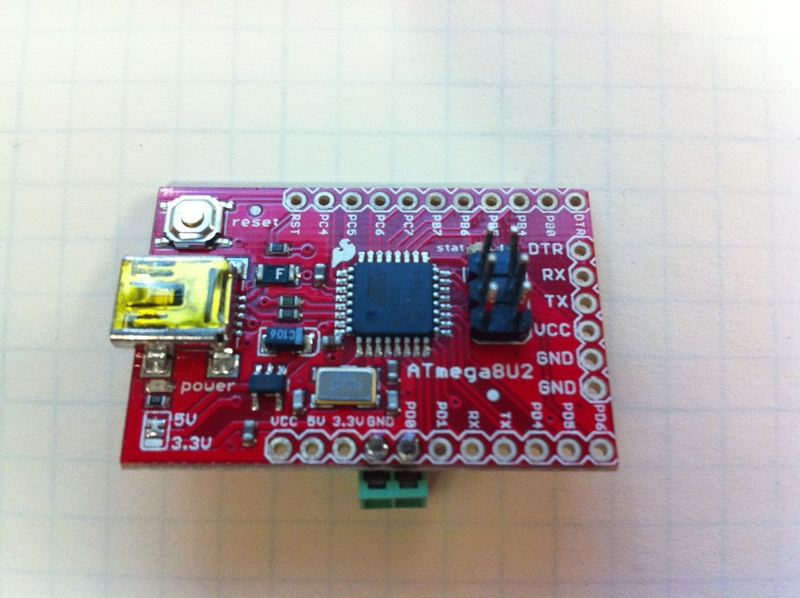
\includegraphics[width=\columnwidth]{microcontroller.jpg}
\end{center}
\caption{Photo of microcontroller terminal block.}
\label{microcontroller}
\end{figure}

\begin{figure}[]
\begin{center}
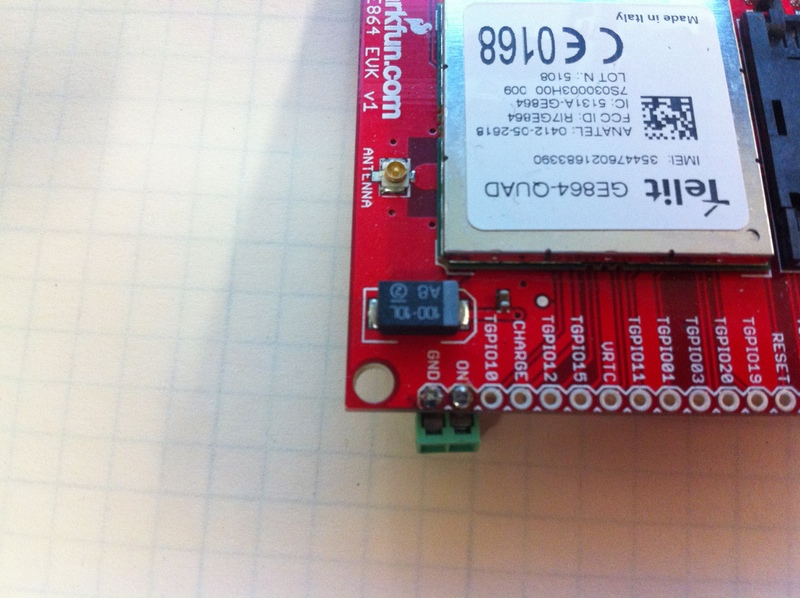
\includegraphics[width=\columnwidth]{modem_unit.jpg}
\end{center}
\caption{Photo of modem terminal block.}
\label{modem_unit}
\end{figure}

\begin{figure}[]
\begin{center}
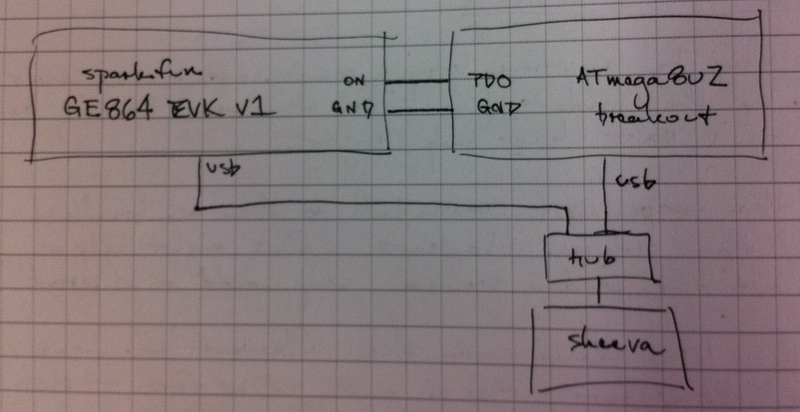
\includegraphics[width=\columnwidth]{schematic.jpg}
\end{center}
\caption{Schematic of connections between boards.}
\label{schematic}
\end{figure}


\end{document}
